% Options for packages loaded elsewhere
\PassOptionsToPackage{unicode}{hyperref}
\PassOptionsToPackage{hyphens}{url}
\PassOptionsToPackage{dvipsnames,svgnames,x11names}{xcolor}
%
\documentclass[
]{article}

\usepackage{amsmath,amssymb}
\usepackage{iftex}
\ifPDFTeX
  \usepackage[T1]{fontenc}
  \usepackage[utf8]{inputenc}
  \usepackage{textcomp} % provide euro and other symbols
\else % if luatex or xetex
  \usepackage{unicode-math}
  \defaultfontfeatures{Scale=MatchLowercase}
  \defaultfontfeatures[\rmfamily]{Ligatures=TeX,Scale=1}
\fi
\usepackage{lmodern}
\ifPDFTeX\else  
    % xetex/luatex font selection
\fi
% Use upquote if available, for straight quotes in verbatim environments
\IfFileExists{upquote.sty}{\usepackage{upquote}}{}
\IfFileExists{microtype.sty}{% use microtype if available
  \usepackage[]{microtype}
  \UseMicrotypeSet[protrusion]{basicmath} % disable protrusion for tt fonts
}{}
\makeatletter
\@ifundefined{KOMAClassName}{% if non-KOMA class
  \IfFileExists{parskip.sty}{%
    \usepackage{parskip}
  }{% else
    \setlength{\parindent}{0pt}
    \setlength{\parskip}{6pt plus 2pt minus 1pt}}
}{% if KOMA class
  \KOMAoptions{parskip=half}}
\makeatother
\usepackage{xcolor}
\setlength{\emergencystretch}{3em} % prevent overfull lines
\setcounter{secnumdepth}{-\maxdimen} % remove section numbering
% Make \paragraph and \subparagraph free-standing
\ifx\paragraph\undefined\else
  \let\oldparagraph\paragraph
  \renewcommand{\paragraph}[1]{\oldparagraph{#1}\mbox{}}
\fi
\ifx\subparagraph\undefined\else
  \let\oldsubparagraph\subparagraph
  \renewcommand{\subparagraph}[1]{\oldsubparagraph{#1}\mbox{}}
\fi

\usepackage{color}
\usepackage{fancyvrb}
\newcommand{\VerbBar}{|}
\newcommand{\VERB}{\Verb[commandchars=\\\{\}]}
\DefineVerbatimEnvironment{Highlighting}{Verbatim}{commandchars=\\\{\}}
% Add ',fontsize=\small' for more characters per line
\usepackage{framed}
\definecolor{shadecolor}{RGB}{241,243,245}
\newenvironment{Shaded}{\begin{snugshade}}{\end{snugshade}}
\newcommand{\AlertTok}[1]{\textcolor[rgb]{0.68,0.00,0.00}{#1}}
\newcommand{\AnnotationTok}[1]{\textcolor[rgb]{0.37,0.37,0.37}{#1}}
\newcommand{\AttributeTok}[1]{\textcolor[rgb]{0.40,0.45,0.13}{#1}}
\newcommand{\BaseNTok}[1]{\textcolor[rgb]{0.68,0.00,0.00}{#1}}
\newcommand{\BuiltInTok}[1]{\textcolor[rgb]{0.00,0.23,0.31}{#1}}
\newcommand{\CharTok}[1]{\textcolor[rgb]{0.13,0.47,0.30}{#1}}
\newcommand{\CommentTok}[1]{\textcolor[rgb]{0.37,0.37,0.37}{#1}}
\newcommand{\CommentVarTok}[1]{\textcolor[rgb]{0.37,0.37,0.37}{\textit{#1}}}
\newcommand{\ConstantTok}[1]{\textcolor[rgb]{0.56,0.35,0.01}{#1}}
\newcommand{\ControlFlowTok}[1]{\textcolor[rgb]{0.00,0.23,0.31}{#1}}
\newcommand{\DataTypeTok}[1]{\textcolor[rgb]{0.68,0.00,0.00}{#1}}
\newcommand{\DecValTok}[1]{\textcolor[rgb]{0.68,0.00,0.00}{#1}}
\newcommand{\DocumentationTok}[1]{\textcolor[rgb]{0.37,0.37,0.37}{\textit{#1}}}
\newcommand{\ErrorTok}[1]{\textcolor[rgb]{0.68,0.00,0.00}{#1}}
\newcommand{\ExtensionTok}[1]{\textcolor[rgb]{0.00,0.23,0.31}{#1}}
\newcommand{\FloatTok}[1]{\textcolor[rgb]{0.68,0.00,0.00}{#1}}
\newcommand{\FunctionTok}[1]{\textcolor[rgb]{0.28,0.35,0.67}{#1}}
\newcommand{\ImportTok}[1]{\textcolor[rgb]{0.00,0.46,0.62}{#1}}
\newcommand{\InformationTok}[1]{\textcolor[rgb]{0.37,0.37,0.37}{#1}}
\newcommand{\KeywordTok}[1]{\textcolor[rgb]{0.00,0.23,0.31}{#1}}
\newcommand{\NormalTok}[1]{\textcolor[rgb]{0.00,0.23,0.31}{#1}}
\newcommand{\OperatorTok}[1]{\textcolor[rgb]{0.37,0.37,0.37}{#1}}
\newcommand{\OtherTok}[1]{\textcolor[rgb]{0.00,0.23,0.31}{#1}}
\newcommand{\PreprocessorTok}[1]{\textcolor[rgb]{0.68,0.00,0.00}{#1}}
\newcommand{\RegionMarkerTok}[1]{\textcolor[rgb]{0.00,0.23,0.31}{#1}}
\newcommand{\SpecialCharTok}[1]{\textcolor[rgb]{0.37,0.37,0.37}{#1}}
\newcommand{\SpecialStringTok}[1]{\textcolor[rgb]{0.13,0.47,0.30}{#1}}
\newcommand{\StringTok}[1]{\textcolor[rgb]{0.13,0.47,0.30}{#1}}
\newcommand{\VariableTok}[1]{\textcolor[rgb]{0.07,0.07,0.07}{#1}}
\newcommand{\VerbatimStringTok}[1]{\textcolor[rgb]{0.13,0.47,0.30}{#1}}
\newcommand{\WarningTok}[1]{\textcolor[rgb]{0.37,0.37,0.37}{\textit{#1}}}

\providecommand{\tightlist}{%
  \setlength{\itemsep}{0pt}\setlength{\parskip}{0pt}}\usepackage{longtable,booktabs,array}
\usepackage{calc} % for calculating minipage widths
% Correct order of tables after \paragraph or \subparagraph
\usepackage{etoolbox}
\makeatletter
\patchcmd\longtable{\par}{\if@noskipsec\mbox{}\fi\par}{}{}
\makeatother
% Allow footnotes in longtable head/foot
\IfFileExists{footnotehyper.sty}{\usepackage{footnotehyper}}{\usepackage{footnote}}
\makesavenoteenv{longtable}
\usepackage{graphicx}
\makeatletter
\def\maxwidth{\ifdim\Gin@nat@width>\linewidth\linewidth\else\Gin@nat@width\fi}
\def\maxheight{\ifdim\Gin@nat@height>\textheight\textheight\else\Gin@nat@height\fi}
\makeatother
% Scale images if necessary, so that they will not overflow the page
% margins by default, and it is still possible to overwrite the defaults
% using explicit options in \includegraphics[width, height, ...]{}
\setkeys{Gin}{width=\maxwidth,height=\maxheight,keepaspectratio}
% Set default figure placement to htbp
\makeatletter
\def\fps@figure{htbp}
\makeatother

\makeatletter
\makeatother
\makeatletter
\makeatother
\makeatletter
\@ifpackageloaded{caption}{}{\usepackage{caption}}
\AtBeginDocument{%
\ifdefined\contentsname
  \renewcommand*\contentsname{Table of contents}
\else
  \newcommand\contentsname{Table of contents}
\fi
\ifdefined\listfigurename
  \renewcommand*\listfigurename{List of Figures}
\else
  \newcommand\listfigurename{List of Figures}
\fi
\ifdefined\listtablename
  \renewcommand*\listtablename{List of Tables}
\else
  \newcommand\listtablename{List of Tables}
\fi
\ifdefined\figurename
  \renewcommand*\figurename{Figure}
\else
  \newcommand\figurename{Figure}
\fi
\ifdefined\tablename
  \renewcommand*\tablename{Table}
\else
  \newcommand\tablename{Table}
\fi
}
\@ifpackageloaded{float}{}{\usepackage{float}}
\floatstyle{ruled}
\@ifundefined{c@chapter}{\newfloat{codelisting}{h}{lop}}{\newfloat{codelisting}{h}{lop}[chapter]}
\floatname{codelisting}{Listing}
\newcommand*\listoflistings{\listof{codelisting}{List of Listings}}
\makeatother
\makeatletter
\@ifpackageloaded{caption}{}{\usepackage{caption}}
\@ifpackageloaded{subcaption}{}{\usepackage{subcaption}}
\makeatother
\makeatletter
\@ifpackageloaded{tcolorbox}{}{\usepackage[skins,breakable]{tcolorbox}}
\makeatother
\makeatletter
\@ifundefined{shadecolor}{\definecolor{shadecolor}{rgb}{.97, .97, .97}}
\makeatother
\makeatletter
\makeatother
\makeatletter
\makeatother
\ifLuaTeX
  \usepackage{selnolig}  % disable illegal ligatures
\fi
\IfFileExists{bookmark.sty}{\usepackage{bookmark}}{\usepackage{hyperref}}
\IfFileExists{xurl.sty}{\usepackage{xurl}}{} % add URL line breaks if available
\urlstyle{same} % disable monospaced font for URLs
\hypersetup{
  pdftitle={Biostat 203B Homework 1},
  pdfauthor={Wenqiang Ge ID:106371961},
  colorlinks=true,
  linkcolor={blue},
  filecolor={Maroon},
  citecolor={Blue},
  urlcolor={Blue},
  pdfcreator={LaTeX via pandoc}}

\title{Biostat 203B Homework 1}
\usepackage{etoolbox}
\makeatletter
\providecommand{\subtitle}[1]{% add subtitle to \maketitle
  \apptocmd{\@title}{\par {\large #1 \par}}{}{}
}
\makeatother
\subtitle{Due Jan 24, 2025 @ 11:59PM}
\author{Wenqiang Ge ID:106371961}
\date{}

\begin{document}
\maketitle
\ifdefined\Shaded\renewenvironment{Shaded}{\begin{tcolorbox}[frame hidden, borderline west={3pt}{0pt}{shadecolor}, boxrule=0pt, interior hidden, enhanced, breakable, sharp corners]}{\end{tcolorbox}}\fi

\renewcommand*\contentsname{Table of contents}
{
\hypersetup{linkcolor=}
\setcounter{tocdepth}{2}
\tableofcontents
}
Display machine information for reproducibility:

\begin{Shaded}
\begin{Highlighting}[]
\FunctionTok{sessionInfo}\NormalTok{()}
\end{Highlighting}
\end{Shaded}

\begin{verbatim}
R version 4.4.2 (2024-10-31)
Platform: x86_64-pc-linux-gnu
Running under: Ubuntu 24.04.1 LTS

Matrix products: default
BLAS:   /usr/lib/x86_64-linux-gnu/blas/libblas.so.3.12.0 
LAPACK: /usr/lib/x86_64-linux-gnu/lapack/liblapack.so.3.12.0

locale:
 [1] LC_CTYPE=C.UTF-8       LC_NUMERIC=C           LC_TIME=C.UTF-8       
 [4] LC_COLLATE=C.UTF-8     LC_MONETARY=C.UTF-8    LC_MESSAGES=C.UTF-8   
 [7] LC_PAPER=C.UTF-8       LC_NAME=C              LC_ADDRESS=C          
[10] LC_TELEPHONE=C         LC_MEASUREMENT=C.UTF-8 LC_IDENTIFICATION=C   

time zone: America/Los_Angeles
tzcode source: system (glibc)

attached base packages:
[1] stats     graphics  grDevices utils     datasets  methods   base     

loaded via a namespace (and not attached):
 [1] compiler_4.4.2    fastmap_1.2.0     cli_3.6.3         tools_4.4.2      
 [5] htmltools_0.5.8.1 rstudioapi_0.17.1 yaml_2.3.10       rmarkdown_2.29   
 [9] knitr_1.49        jsonlite_1.8.9    xfun_0.50         digest_0.6.37    
[13] rlang_1.1.5       evaluate_1.0.3   
\end{verbatim}

\hypertarget{q1.-gitgithub}{%
\subsection{Q1. Git/GitHub}\label{q1.-gitgithub}}

\textbf{No handwritten homework reports are accepted for this course.}
We work with Git and GitHub. Efficient and abundant use of Git, e.g.,
frequent and well-documented commits, is an important criterion for
grading your homework.

\begin{enumerate}
\def\labelenumi{\arabic{enumi}.}
\item
  Apply for the \href{https://education.github.com/pack}{Student
  Developer Pack} at GitHub using your UCLA email. You'll get GitHub Pro
  account for free (unlimited public and private repositories).
\item
  Create a \textbf{private} repository \texttt{biostat-203b-2025-winter}
  and add \texttt{Hua-Zhou} and TA team (\texttt{Tomoki-Okuno} for Lec
  1; \texttt{parsajamshidian} and \texttt{BowenZhang2001} for Lec 82) as
  your collaborators with write permission.
\item
  Top directories of the repository should be \texttt{hw1},
  \texttt{hw2}, \ldots{} Maintain two branches \texttt{main} and
  \texttt{develop}. The \texttt{develop} branch will be your main
  playground, the place where you develop solution (code) to homework
  problems and write up report. The \texttt{main} branch will be your
  presentation area. Submit your homework files (Quarto file
  \texttt{qmd}, \texttt{html} file converted by Quarto, all code and
  extra data sets to reproduce results) in the \texttt{main} branch.
\item
  After each homework due date, course reader and instructor will check
  out your \texttt{main} branch for grading. Tag each of your homework
  submissions with tag names \texttt{hw1}, \texttt{hw2}, \ldots{}
  Tagging time will be used as your submission time. That means if you
  tag your \texttt{hw1} submission after deadline, penalty points will
  be deducted for late submission.
\item
  After this course, you can make this repository public and use it to
  demonstrate your skill sets on job market.
\end{enumerate}

\textbf{Solution:}

Done!

\hypertarget{q2.-data-ethics-training}{%
\subsection{Q2. Data ethics training}\label{q2.-data-ethics-training}}

This exercise (and later in this course) uses the
\href{https://physionet.org/content/mimiciv/3.1/}{MIMIC-IV data v3.1}, a
freely accessible critical care database developed by the MIT Lab for
Computational Physiology. Follow the instructions at
\url{https://mimic.mit.edu/docs/gettingstarted/} to (1) complete the
CITI \texttt{Data\ or\ Specimens\ Only\ Research} course and (2) obtain
the PhysioNet credential for using the MIMIC-IV data. Display the
verification links to your completion report and completion certificate
here. \textbf{You must complete Q2 before working on the remaining
questions.} (Hint: The CITI training takes a few hours and the PhysioNet
credentialing takes a couple days; do not leave it to the last minute.)

\textbf{Solution:}

Completion Report Link:
\url{https://www.citiprogram.org/verify/?kcc436586-af5d-4128-bb91-ef37f2326698-67297842}

Completion Certificate
Link:\url{https://www.citiprogram.org/verify/?w7ddecc3c-d853-4bc4-95ec-c08cd3268665-67297842}

sessionInfo()

\hypertarget{q3.-linux-shell-commands}{%
\subsection{Q3. Linux Shell Commands}\label{q3.-linux-shell-commands}}

\begin{enumerate}
\def\labelenumi{\arabic{enumi}.}
\tightlist
\item
  Make the MIMIC-IV v3.1 data available at location
  \texttt{\textasciitilde{}/mimic}. The output of the
  \texttt{ls\ -l\ \textasciitilde{}/mimic} command should be similar to
  the below (from my laptop).
\end{enumerate}

\begin{Shaded}
\begin{Highlighting}[]
\CommentTok{\# content of mimic folder}
\FunctionTok{ls} \AttributeTok{{-}l}\NormalTok{ \textasciitilde{}/mimic/}
\end{Highlighting}
\end{Shaded}

\begin{verbatim}
total 28
-rwxrwxrwx 1 gewenqiang gewenqiang 15199 Jan 16 19:00 CHANGELOG.txt
-rwxrwxrwx 1 gewenqiang gewenqiang  2518 Jan 16 19:00 LICENSE.txt
-rwxrwxrwx 1 gewenqiang gewenqiang  2884 Jan 16 19:00 SHA256SUMS.txt
drwxrwxrwx 1 gewenqiang gewenqiang  4096 Jan 23 18:37 hosp
drwxrwxrwx 1 gewenqiang gewenqiang  4096 Jan 16 19:02 icu
-rwxrwxrwx 1 gewenqiang gewenqiang   789 Jan 16 19:00 index.html
\end{verbatim}

Refer to the documentation
\url{https://physionet.org/content/mimiciv/3.1/} for details of data
files. Do \textbf{not} put these data files into Git; they are big. Do
\textbf{not} copy them into your directory. Do \textbf{not} decompress
the gz data files. These create unnecessary big files and are not
big-data-friendly practices. Read from the data folder
\texttt{\textasciitilde{}/mimic} directly in following exercises.

Use Bash commands to answer following questions.

\begin{enumerate}
\def\labelenumi{\arabic{enumi}.}
\setcounter{enumi}{1}
\tightlist
\item
  Display the contents in the folders \texttt{hosp} and \texttt{icu}
  using Bash command \texttt{ls\ -l}. Why are these data files
  distributed as \texttt{.csv.gz} files instead of \texttt{.csv} (comma
  separated values) files? Read the page
  \url{https://mimic.mit.edu/docs/iv/} to understand what's in each
  folder.
\end{enumerate}

\textbf{Solution:}

\begin{Shaded}
\begin{Highlighting}[]
\FunctionTok{ls} \AttributeTok{{-}l}\NormalTok{ \textasciitilde{}/mimic/hosp}
\end{Highlighting}
\end{Shaded}

\begin{verbatim}
total 6153128
-rwxrwxrwx 1 gewenqiang gewenqiang   19928140 Jan 16 19:00 admissions.csv.gz
-rwxrwxrwx 1 gewenqiang gewenqiang     427554 Jan 16 19:00 d_hcpcs.csv.gz
-rwxrwxrwx 1 gewenqiang gewenqiang     876360 Jan 16 19:00 d_icd_diagnoses.csv.gz
-rwxrwxrwx 1 gewenqiang gewenqiang     589186 Jan 16 19:00 d_icd_procedures.csv.gz
-rwxrwxrwx 1 gewenqiang gewenqiang      13169 Jan 16 19:00 d_labitems.csv.gz
-rwxrwxrwx 1 gewenqiang gewenqiang   33564802 Jan 16 19:00 diagnoses_icd.csv.gz
-rwxrwxrwx 1 gewenqiang gewenqiang    9743908 Jan 16 19:00 drgcodes.csv.gz
-rwxrwxrwx 1 gewenqiang gewenqiang  811305629 Jan 16 19:00 emar.csv.gz
-rwxrwxrwx 1 gewenqiang gewenqiang  748158322 Jan 16 19:00 emar_detail.csv.gz
-rwxrwxrwx 1 gewenqiang gewenqiang    2162335 Jan 16 19:00 hcpcsevents.csv.gz
-rwxrwxrwx 1 gewenqiang gewenqiang       2907 Jan 16 19:00 index.html
-rwxrwxrwx 1 gewenqiang gewenqiang 2592909134 Jan 16 19:01 labevents.csv.gz
-rwxrwxrwx 1 gewenqiang gewenqiang  117644075 Jan 16 19:01 microbiologyevents.csv.gz
-rwxrwxrwx 1 gewenqiang gewenqiang   44069351 Jan 16 19:01 omr.csv.gz
-rwxrwxrwx 1 gewenqiang gewenqiang    2835586 Jan 16 19:01 patients.csv.gz
-rwxrwxrwx 1 gewenqiang gewenqiang  525708076 Jan 16 19:01 pharmacy.csv.gz
-rwxrwxrwx 1 gewenqiang gewenqiang  666594177 Jan 16 19:01 poe.csv.gz
-rwxrwxrwx 1 gewenqiang gewenqiang   55267894 Jan 16 19:01 poe_detail.csv.gz
-rwxrwxrwx 1 gewenqiang gewenqiang  606298611 Jan 16 19:01 prescriptions.csv.gz
-rwxrwxrwx 1 gewenqiang gewenqiang    7777324 Jan 16 19:01 procedures_icd.csv.gz
-rwxrwxrwx 1 gewenqiang gewenqiang     127330 Jan 16 19:01 provider.csv.gz
-rwxrwxrwx 1 gewenqiang gewenqiang    8569241 Jan 16 19:01 services.csv.gz
-rwxrwxrwx 1 gewenqiang gewenqiang   46185771 Jan 16 19:01 transfers.csv.gz
\end{verbatim}

\begin{Shaded}
\begin{Highlighting}[]
\FunctionTok{ls} \AttributeTok{{-}l}\NormalTok{ \textasciitilde{}/mimic/icu}
\end{Highlighting}
\end{Shaded}

\begin{verbatim}
total 4253396
-rwxrwxrwx 1 gewenqiang gewenqiang      41566 Jan 16 19:01 caregiver.csv.gz
-rwxrwxrwx 1 gewenqiang gewenqiang 3502392765 Jan 16 19:02 chartevents.csv.gz
-rwxrwxrwx 1 gewenqiang gewenqiang      58741 Jan 16 19:02 d_items.csv.gz
-rwxrwxrwx 1 gewenqiang gewenqiang   63481196 Jan 16 19:02 datetimeevents.csv.gz
-rwxrwxrwx 1 gewenqiang gewenqiang    3342355 Jan 16 19:02 icustays.csv.gz
-rwxrwxrwx 1 gewenqiang gewenqiang       1336 Jan 16 19:02 index.html
-rwxrwxrwx 1 gewenqiang gewenqiang  311642048 Jan 16 19:02 ingredientevents.csv.gz
-rwxrwxrwx 1 gewenqiang gewenqiang  401088206 Jan 16 19:02 inputevents.csv.gz
-rwxrwxrwx 1 gewenqiang gewenqiang   49307639 Jan 16 19:02 outputevents.csv.gz
-rwxrwxrwx 1 gewenqiang gewenqiang   24096834 Jan 16 19:02 procedureevents.csv.gz
\end{verbatim}

Compressed files save disk space as \texttt{.gz} files are smaller than
raw \texttt{.csv} files. This will help to reduce network bandwidth
usage and time required to download or transfer files. In addition,
compression ensures the original data remains unaltered.

\begin{enumerate}
\def\labelenumi{\arabic{enumi}.}
\setcounter{enumi}{2}
\tightlist
\item
  Briefly describe what Bash commands \texttt{zcat}, \texttt{zless},
  \texttt{zmore}, and \texttt{zgrep} do.
\end{enumerate}

zcat: Outputs the contents of a compressed .gz file to the standard
output without decompressing it to disk.

\textbf{Solution:}

zless: Allows you to view a compressed .gz file interactively, similar
to less for uncompressed files.

zmore: Similar to zless, but works like more, showing the file in a
paginated manner.

zgrep: Searches for a pattern inside a .gz compressed file, equivalent
to grep for uncompressed files.

\begin{enumerate}
\def\labelenumi{\arabic{enumi}.}
\setcounter{enumi}{3}
\tightlist
\item
  (Looping in Bash) What's the output of the following bash script?
\end{enumerate}

\begin{Shaded}
\begin{Highlighting}[]
\ControlFlowTok{for}\NormalTok{ datafile }\KeywordTok{in}\NormalTok{ \textasciitilde{}/mimic/hosp/}\DataTypeTok{\{a}\OperatorTok{,}\DataTypeTok{l}\OperatorTok{,}\DataTypeTok{pa\}}\PreprocessorTok{*}\NormalTok{.gz}
\ControlFlowTok{do}
  \FunctionTok{ls} \AttributeTok{{-}l} \VariableTok{$datafile}
\ControlFlowTok{done}
\end{Highlighting}
\end{Shaded}

Display the number of lines in each data file using a similar loop.
(Hint: combine linux commands \texttt{zcat\ \textless{}} and
\texttt{wc\ -l}.)

\textbf{Solution:}

\begin{Shaded}
\begin{Highlighting}[]
\ControlFlowTok{for}\NormalTok{ datafile }\KeywordTok{in}\NormalTok{ \textasciitilde{}/mimic/hosp/}\PreprocessorTok{*}\NormalTok{.gz}
\ControlFlowTok{do} 
  \BuiltInTok{echo} \StringTok{"File: }\VariableTok{$datafile}\StringTok{"}
  \FunctionTok{zcat} \StringTok{"}\VariableTok{$datafile}\StringTok{"} \KeywordTok{|} \FunctionTok{wc} \AttributeTok{{-}l}
\ControlFlowTok{done}
\end{Highlighting}
\end{Shaded}

\begin{verbatim}
File: /home/gewenqiang/mimic/hosp/admissions.csv.gz
546029
File: /home/gewenqiang/mimic/hosp/d_hcpcs.csv.gz
89209
File: /home/gewenqiang/mimic/hosp/d_icd_diagnoses.csv.gz
112108
File: /home/gewenqiang/mimic/hosp/d_icd_procedures.csv.gz
86424
File: /home/gewenqiang/mimic/hosp/d_labitems.csv.gz
1651
File: /home/gewenqiang/mimic/hosp/diagnoses_icd.csv.gz
6364489
File: /home/gewenqiang/mimic/hosp/drgcodes.csv.gz
761857
File: /home/gewenqiang/mimic/hosp/emar.csv.gz
42808594
File: /home/gewenqiang/mimic/hosp/emar_detail.csv.gz
87371065
File: /home/gewenqiang/mimic/hosp/hcpcsevents.csv.gz
186075
File: /home/gewenqiang/mimic/hosp/labevents.csv.gz
158374765
File: /home/gewenqiang/mimic/hosp/microbiologyevents.csv.gz
3988225
File: /home/gewenqiang/mimic/hosp/omr.csv.gz
7753028
File: /home/gewenqiang/mimic/hosp/patients.csv.gz
364628
File: /home/gewenqiang/mimic/hosp/pharmacy.csv.gz
17847568
File: /home/gewenqiang/mimic/hosp/poe.csv.gz
52212110
File: /home/gewenqiang/mimic/hosp/poe_detail.csv.gz
8504983
File: /home/gewenqiang/mimic/hosp/prescriptions.csv.gz
20292612
File: /home/gewenqiang/mimic/hosp/procedures_icd.csv.gz
859656
File: /home/gewenqiang/mimic/hosp/provider.csv.gz
42245
File: /home/gewenqiang/mimic/hosp/services.csv.gz
593072
File: /home/gewenqiang/mimic/hosp/transfers.csv.gz
2413582
\end{verbatim}

\begin{Shaded}
\begin{Highlighting}[]
\ControlFlowTok{for}\NormalTok{ datafile }\KeywordTok{in}\NormalTok{ \textasciitilde{}/mimic/icu/}\PreprocessorTok{*}\NormalTok{.gz}
\ControlFlowTok{do} 
  \BuiltInTok{echo} \StringTok{"File: }\VariableTok{$datafile}\StringTok{"}
  \FunctionTok{zcat} \StringTok{"}\VariableTok{$datafile}\StringTok{"} \KeywordTok{|} \FunctionTok{wc} \AttributeTok{{-}l}
\ControlFlowTok{done}
\end{Highlighting}
\end{Shaded}

\begin{verbatim}
File: /home/gewenqiang/mimic/icu/caregiver.csv.gz
17985
File: /home/gewenqiang/mimic/icu/chartevents.csv.gz
432997492
File: /home/gewenqiang/mimic/icu/d_items.csv.gz
4096
File: /home/gewenqiang/mimic/icu/datetimeevents.csv.gz
9979762
File: /home/gewenqiang/mimic/icu/icustays.csv.gz
94459
File: /home/gewenqiang/mimic/icu/ingredientevents.csv.gz
14253481
File: /home/gewenqiang/mimic/icu/inputevents.csv.gz
10953714
File: /home/gewenqiang/mimic/icu/outputevents.csv.gz
5359396
File: /home/gewenqiang/mimic/icu/procedureevents.csv.gz
808707
\end{verbatim}

\begin{enumerate}
\def\labelenumi{\arabic{enumi}.}
\setcounter{enumi}{4}
\tightlist
\item
  Display the first few lines of \texttt{admissions.csv.gz}. How many
  rows are in this data file, excluding the header line? Each
  \texttt{hadm\_id} identifies a hospitalization. How many
  hospitalizations are in this data file? How many unique patients
  (identified by \texttt{subject\_id}) are in this da`ta file? Do they
  match the number of patients listed in the \texttt{patients.csv.gz}
  file? (Hint: combine Linux commands \texttt{zcat\ \textless{}},
  \texttt{head}/\texttt{tail}, \texttt{awk}, \texttt{sort},
  \texttt{uniq}, \texttt{wc}, and so on.)
\end{enumerate}

\textbf{Solution:}

\begin{Shaded}
\begin{Highlighting}[]
\FunctionTok{zcat}\NormalTok{ \textasciitilde{}/mimic/hosp/admissions.csv.gz }\KeywordTok{|} \FunctionTok{head}
\end{Highlighting}
\end{Shaded}

\begin{verbatim}
subject_id,hadm_id,admittime,dischtime,deathtime,admission_type,admit_provider_id,admission_location,discharge_location,insurance,language,marital_status,race,edregtime,edouttime,hospital_expire_flag
10000032,22595853,2180-05-06 22:23:00,2180-05-07 17:15:00,,URGENT,P49AFC,TRANSFER FROM HOSPITAL,HOME,Medicaid,English,WIDOWED,WHITE,2180-05-06 19:17:00,2180-05-06 23:30:00,0
10000032,22841357,2180-06-26 18:27:00,2180-06-27 18:49:00,,EW EMER.,P784FA,EMERGENCY ROOM,HOME,Medicaid,English,WIDOWED,WHITE,2180-06-26 15:54:00,2180-06-26 21:31:00,0
10000032,25742920,2180-08-05 23:44:00,2180-08-07 17:50:00,,EW EMER.,P19UTS,EMERGENCY ROOM,HOSPICE,Medicaid,English,WIDOWED,WHITE,2180-08-05 20:58:00,2180-08-06 01:44:00,0
10000032,29079034,2180-07-23 12:35:00,2180-07-25 17:55:00,,EW EMER.,P06OTX,EMERGENCY ROOM,HOME,Medicaid,English,WIDOWED,WHITE,2180-07-23 05:54:00,2180-07-23 14:00:00,0
10000068,25022803,2160-03-03 23:16:00,2160-03-04 06:26:00,,EU OBSERVATION,P39NWO,EMERGENCY ROOM,,,English,SINGLE,WHITE,2160-03-03 21:55:00,2160-03-04 06:26:00,0
10000084,23052089,2160-11-21 01:56:00,2160-11-25 14:52:00,,EW EMER.,P42H7G,WALK-IN/SELF REFERRAL,HOME HEALTH CARE,Medicare,English,MARRIED,WHITE,2160-11-20 20:36:00,2160-11-21 03:20:00,0
10000084,29888819,2160-12-28 05:11:00,2160-12-28 16:07:00,,EU OBSERVATION,P35NE4,PHYSICIAN REFERRAL,,Medicare,English,MARRIED,WHITE,2160-12-27 18:32:00,2160-12-28 16:07:00,0
10000108,27250926,2163-09-27 23:17:00,2163-09-28 09:04:00,,EU OBSERVATION,P40JML,EMERGENCY ROOM,,,English,SINGLE,WHITE,2163-09-27 16:18:00,2163-09-28 09:04:00,0
10000117,22927623,2181-11-15 02:05:00,2181-11-15 14:52:00,,EU OBSERVATION,P47EY8,EMERGENCY ROOM,,Medicaid,English,DIVORCED,WHITE,2181-11-14 21:51:00,2181-11-15 09:57:00,0
\end{verbatim}

\begin{Shaded}
\begin{Highlighting}[]
\FunctionTok{zcat}\NormalTok{ \textasciitilde{}/mimic/hosp/admissions.csv.gz }\KeywordTok{|} \FunctionTok{tail} \AttributeTok{{-}n+2} \KeywordTok{|} \DataTypeTok{\textbackslash{}}
  \FunctionTok{awk} \AttributeTok{{-}F,} \StringTok{\textquotesingle{}\{print $2\}\textquotesingle{}} \KeywordTok{|} \FunctionTok{wc} \AttributeTok{{-}l}

\FunctionTok{zcat}\NormalTok{ \textasciitilde{}/mimic/hosp/admissions.csv.gz }\KeywordTok{|} \FunctionTok{tail} \AttributeTok{{-}n+2} \KeywordTok{|} \DataTypeTok{\textbackslash{}}
  \FunctionTok{awk} \AttributeTok{{-}F,} \StringTok{\textquotesingle{}\{print $2\}\textquotesingle{}} \KeywordTok{|} \FunctionTok{sort} \KeywordTok{|} \FunctionTok{uniq} \KeywordTok{|} \FunctionTok{wc} \AttributeTok{{-}l}

\FunctionTok{zcat}\NormalTok{ \textasciitilde{}/mimic/hosp/admissions.csv.gz }\KeywordTok{|} \FunctionTok{tail} \AttributeTok{{-}n+2} \KeywordTok{|} \DataTypeTok{\textbackslash{}}
  \FunctionTok{awk} \AttributeTok{{-}F,} \StringTok{\textquotesingle{}\{print $1\}\textquotesingle{}} \KeywordTok{|} \FunctionTok{sort} \KeywordTok{|} \FunctionTok{uniq} \KeywordTok{|} \FunctionTok{wc} \AttributeTok{{-}l}

\FunctionTok{zcat}\NormalTok{ \textasciitilde{}/mimic/hosp/patients.csv.gz }\KeywordTok{|} \FunctionTok{tail} \AttributeTok{{-}n+2} \KeywordTok{|} \DataTypeTok{\textbackslash{}}
  \FunctionTok{awk} \AttributeTok{{-}F,} \StringTok{\textquotesingle{}\{print $1\}\textquotesingle{}} \KeywordTok{|} \FunctionTok{sort} \KeywordTok{|} \FunctionTok{uniq} \KeywordTok{|} \FunctionTok{wc} \AttributeTok{{-}l}
\end{Highlighting}
\end{Shaded}

\begin{verbatim}
546028
546028
223452
364627
\end{verbatim}

There are 546028 lines in the adimission.csv.gz.

546028 hospitalizations; 223452 unique patients.

There are 364627 unique patients listed in the patients.csv.gz file.
They are not matched.

\begin{enumerate}
\def\labelenumi{\arabic{enumi}.}
\setcounter{enumi}{5}
\tightlist
\item
  What are the possible values taken by each of the variable
  \texttt{admission\_type}, \texttt{admission\_location},
  \texttt{insurance}, and \texttt{ethnicity}? Also report the count for
  each unique value of these variables in decreasing order. (Hint:
  combine Linux commands \texttt{zcat}, \texttt{head}/\texttt{tail},
  \texttt{awk}, \texttt{uniq\ -c}, \texttt{wc}, \texttt{sort}, and so
  on; skip the header line.)
\end{enumerate}

\textbf{Solution:}

\begin{Shaded}
\begin{Highlighting}[]
\FunctionTok{zcat}\NormalTok{ \textasciitilde{}/mimic/hosp/admissions.csv.gz }\KeywordTok{|} \FunctionTok{head} \AttributeTok{{-}n}\NormalTok{ 1 }\KeywordTok{|} \FunctionTok{tr} \StringTok{\textquotesingle{},\textquotesingle{}} \StringTok{\textquotesingle{}\textbackslash{}n\textquotesingle{}} \KeywordTok{|} \FunctionTok{nl}
\end{Highlighting}
\end{Shaded}

\begin{verbatim}
     1  subject_id
     2  hadm_id
     3  admittime
     4  dischtime
     5  deathtime
     6  admission_type
     7  admit_provider_id
     8  admission_location
     9  discharge_location
    10  insurance
    11  language
    12  marital_status
    13  race
    14  edregtime
    15  edouttime
    16  hospital_expire_flag
\end{verbatim}

\begin{Shaded}
\begin{Highlighting}[]
\FunctionTok{zcat}\NormalTok{ \textasciitilde{}/mimic/hosp/admissions.csv.gz }\KeywordTok{|} \FunctionTok{tail} \AttributeTok{{-}n+2} \KeywordTok{|} \DataTypeTok{\textbackslash{}}
  \FunctionTok{awk} \AttributeTok{{-}F} \StringTok{\textquotesingle{},\textquotesingle{}} \StringTok{\textquotesingle{}\{print $6\}\textquotesingle{}} \KeywordTok{|} \FunctionTok{sort} \KeywordTok{|} \FunctionTok{uniq} \AttributeTok{{-}c} \KeywordTok{|} \FunctionTok{sort} \AttributeTok{{-}nr}

\FunctionTok{zcat}\NormalTok{ \textasciitilde{}/mimic/hosp/admissions.csv.gz }\KeywordTok{|} \FunctionTok{tail} \AttributeTok{{-}n+2} \KeywordTok{|} \DataTypeTok{\textbackslash{}}
  \FunctionTok{awk} \AttributeTok{{-}F} \StringTok{\textquotesingle{},\textquotesingle{}} \StringTok{\textquotesingle{}\{print $8\}\textquotesingle{}} \KeywordTok{|} \FunctionTok{sort} \KeywordTok{|} \FunctionTok{uniq} \AttributeTok{{-}c} \KeywordTok{|} \FunctionTok{sort} \AttributeTok{{-}nr}

\FunctionTok{zcat}\NormalTok{ \textasciitilde{}/mimic/hosp/admissions.csv.gz }\KeywordTok{|} \FunctionTok{tail} \AttributeTok{{-}n+2} \KeywordTok{|} \DataTypeTok{\textbackslash{}}
  \FunctionTok{awk} \AttributeTok{{-}F} \StringTok{\textquotesingle{},\textquotesingle{}} \StringTok{\textquotesingle{}\{print $10\}\textquotesingle{}} \KeywordTok{|} \FunctionTok{sort} \KeywordTok{|} \FunctionTok{uniq} \AttributeTok{{-}c} \KeywordTok{|} \FunctionTok{sort} \AttributeTok{{-}nr}

\FunctionTok{zcat}\NormalTok{ \textasciitilde{}/mimic/hosp/admissions.csv.gz }\KeywordTok{|} \FunctionTok{tail} \AttributeTok{{-}n+2} \KeywordTok{|} \DataTypeTok{\textbackslash{}}
  \FunctionTok{awk} \AttributeTok{{-}F} \StringTok{\textquotesingle{},\textquotesingle{}} \StringTok{\textquotesingle{}\{print $13\}\textquotesingle{}} \KeywordTok{|} \FunctionTok{sort} \KeywordTok{|} \FunctionTok{uniq} \AttributeTok{{-}c} \KeywordTok{|} \FunctionTok{sort} \AttributeTok{{-}nr}
\end{Highlighting}
\end{Shaded}

\begin{verbatim}
 177459 EW EMER.
 119456 EU OBSERVATION
  84437 OBSERVATION ADMIT
  54929 URGENT
  42898 SURGICAL SAME DAY ADMISSION
  24551 DIRECT OBSERVATION
  21973 DIRECT EMER.
  13130 ELECTIVE
   7195 AMBULATORY OBSERVATION
 244179 EMERGENCY ROOM
 163228 PHYSICIAN REFERRAL
  56227 TRANSFER FROM HOSPITAL
  42365 WALK-IN/SELF REFERRAL
  12965 CLINIC REFERRAL
   8518 PROCEDURE SITE
   6317 TRANSFER FROM SKILLED NURSING FACILITY
   5837 INTERNAL TRANSFER TO OR FROM PSYCH
   5734 PACU
    402 INFORMATION NOT AVAILABLE
    255 AMBULATORY SURGERY TRANSFER
      1 
 244576 Medicare
 173399 Private
 104229 Medicaid
  14006 Other
   9355 
    463 No charge
 336538 WHITE
  75482 BLACK/AFRICAN AMERICAN
  19788 OTHER
  13972 WHITE - OTHER EUROPEAN
  13870 UNKNOWN
  10903 HISPANIC/LATINO - PUERTO RICAN
   8287 HISPANIC OR LATINO
   7809 ASIAN
   7644 ASIAN - CHINESE
   6597 WHITE - RUSSIAN
   6205 BLACK/CAPE VERDEAN
   6070 HISPANIC/LATINO - DOMINICAN
   3875 BLACK/CARIBBEAN ISLAND
   3495 BLACK/AFRICAN
   3478 UNABLE TO OBTAIN
   2162 PATIENT DECLINED TO ANSWER
   2082 PORTUGUESE
   1973 ASIAN - SOUTH EAST ASIAN
   1886 WHITE - EASTERN EUROPEAN
   1858 HISPANIC/LATINO - GUATEMALAN
   1661 ASIAN - ASIAN INDIAN
   1526 WHITE - BRAZILIAN
   1320 HISPANIC/LATINO - SALVADORAN
   1247 AMERICAN INDIAN/ALASKA NATIVE
    920 HISPANIC/LATINO - COLUMBIAN
    883 HISPANIC/LATINO - MEXICAN
    774 SOUTH AMERICAN
    725 HISPANIC/LATINO - HONDURAN
    664 ASIAN - KOREAN
    641 HISPANIC/LATINO - CUBAN
    603 HISPANIC/LATINO - CENTRAL AMERICAN
    596 MULTIPLE RACE/ETHNICITY
    494 NATIVE HAWAIIAN OR OTHER PACIFIC ISLANDER
\end{verbatim}

\begin{enumerate}
\def\labelenumi{\arabic{enumi}.}
\setcounter{enumi}{6}
\tightlist
\item
  The \texttt{icusays.csv.gz} file contains all the ICU stays during the
  study period. How many ICU stays, identified by \texttt{stay\_id}, are
  in this data file? How many unique patients, identified by
  \texttt{subject\_id}, are in this data file?
\end{enumerate}

\textbf{Solution:}

\begin{Shaded}
\begin{Highlighting}[]
\FunctionTok{zcat}\NormalTok{ \textasciitilde{}/mimic/icu/icustays.csv.gz }\KeywordTok{|} \FunctionTok{head} \AttributeTok{{-}n}\NormalTok{ 1 }\KeywordTok{|} \FunctionTok{tr} \StringTok{\textquotesingle{},\textquotesingle{}} \StringTok{\textquotesingle{}\textbackslash{}n\textquotesingle{}} \KeywordTok{|}\FunctionTok{nl}
\end{Highlighting}
\end{Shaded}

\begin{verbatim}
     1  subject_id
     2  hadm_id
     3  stay_id
     4  first_careunit
     5  last_careunit
     6  intime
     7  outtime
     8  los
\end{verbatim}

\begin{Shaded}
\begin{Highlighting}[]
\FunctionTok{zcat}\NormalTok{ \textasciitilde{}/mimic/icu/icustays.csv.gz }\KeywordTok{|} \FunctionTok{tail} \AttributeTok{{-}n+2} \KeywordTok{|} \DataTypeTok{\textbackslash{}}
  \FunctionTok{awk} \AttributeTok{{-}F} \StringTok{\textquotesingle{},\textquotesingle{}} \StringTok{\textquotesingle{}\{print $1\}\textquotesingle{}} \KeywordTok{|} \FunctionTok{wc} \AttributeTok{{-}l}

\FunctionTok{zcat}\NormalTok{ \textasciitilde{}/mimic/icu/icustays.csv.gz }\KeywordTok{|} \FunctionTok{tail} \AttributeTok{{-}n+2} \KeywordTok{|} \DataTypeTok{\textbackslash{}}
  \FunctionTok{awk} \AttributeTok{{-}F} \StringTok{\textquotesingle{},\textquotesingle{}} \StringTok{\textquotesingle{}\{print $1\}\textquotesingle{}} \KeywordTok{|} \FunctionTok{sort} \KeywordTok{|} \FunctionTok{uniq} \KeywordTok{|} \FunctionTok{wc} \AttributeTok{{-}l}

\FunctionTok{zcat}\NormalTok{ \textasciitilde{}/mimic/icu/icustays.csv.gz }\KeywordTok{|} \FunctionTok{tail} \AttributeTok{{-}n+2} \KeywordTok{|} \DataTypeTok{\textbackslash{}}
  \FunctionTok{awk} \AttributeTok{{-}F} \StringTok{\textquotesingle{},\textquotesingle{}} \StringTok{\textquotesingle{}\{print $3\}\textquotesingle{}} \KeywordTok{|} \FunctionTok{sort} \KeywordTok{|} \FunctionTok{uniq} \KeywordTok{|} \FunctionTok{wc} \AttributeTok{{-}l}

\FunctionTok{zcat}\NormalTok{ \textasciitilde{}/mimic/icu/icustays.csv.gz }\KeywordTok{|} \FunctionTok{tail} \AttributeTok{{-}n+2} \KeywordTok{|} \DataTypeTok{\textbackslash{}}
  \FunctionTok{awk} \AttributeTok{{-}F} \StringTok{\textquotesingle{},\textquotesingle{}} \StringTok{\textquotesingle{}\{print $1\}\textquotesingle{}} \KeywordTok{|} \FunctionTok{wc} \AttributeTok{{-}l}
\end{Highlighting}
\end{Shaded}

\begin{verbatim}
94458
65366
94458
94458
\end{verbatim}

There are 94458 ICU stays and 65366 unique patients in this data file.

\begin{enumerate}
\def\labelenumi{\arabic{enumi}.}
\setcounter{enumi}{7}
\tightlist
\item
  \emph{To compress, or not to compress. That's the question.} Let's
  focus on the big data file \texttt{labevents.csv.gz}. Compare
  compressed gz file size to the uncompressed file size. Compare the run
  times of
  \texttt{zcat\ \textless{}\ \textasciitilde{}/mimic/labevents.csv.gz\ \textbar{}\ wc\ -l}
  versus \texttt{wc\ -l\ labevents.csv}. Discuss the trade off between
  storage and speed for big data files. (Hint:
  \texttt{gzip\ -dk\ \textless{}\ FILENAME.gz\ \textgreater{}\ ./FILENAME}.
  Remember to delete the large \texttt{labevents.csv} file after the
  exercise.)
\end{enumerate}

\textbf{Solution:}

Comparison of file size:

\begin{Shaded}
\begin{Highlighting}[]
\FunctionTok{gzip} \AttributeTok{{-}dk}\NormalTok{ \textasciitilde{}/mimic/hosp/labevents.csv.gz}
\end{Highlighting}
\end{Shaded}

\begin{Shaded}
\begin{Highlighting}[]
\FunctionTok{ls} \AttributeTok{{-}lh}\NormalTok{ \textasciitilde{}/mimic/hosp/labevents.csv.gz}
\FunctionTok{ls} \AttributeTok{{-}lh}\NormalTok{ \textasciitilde{}/mimic/hosp/labevents.csv}
\end{Highlighting}
\end{Shaded}

\begin{verbatim}
-rwxrwxrwx 1 gewenqiang gewenqiang 2.5G Jan 16 19:01 /home/gewenqiang/mimic/hosp/labevents.csv.gz
-rwxrwxrwx 1 gewenqiang gewenqiang 18G Jan 16 19:01 /home/gewenqiang/mimic/hosp/labevents.csv
\end{verbatim}

Comparison of run times:

\begin{Shaded}
\begin{Highlighting}[]
\BuiltInTok{time}\NormalTok{ zcat \textasciitilde{}/mimic/hosp/labevents.csv.gz }\KeywordTok{|} \FunctionTok{wc} \AttributeTok{{-}l}
\end{Highlighting}
\end{Shaded}

\begin{verbatim}
158374765

real    1m50.148s
user    1m15.779s
sys 0m25.595s
\end{verbatim}

\begin{Shaded}
\begin{Highlighting}[]
\NormalTok{time wc {-}l \textasciitilde{}/mimic/hosp/labevents.csv }
\end{Highlighting}
\end{Shaded}

\begin{Shaded}
\begin{Highlighting}[]
\FunctionTok{rm}\NormalTok{ \textasciitilde{}/mimic/hosp/labevents.csv}
\end{Highlighting}
\end{Shaded}

\textbf{Trade off:} Storage trade-off Compressing files can save a lot
of disk space and reduce network transmission time when moving data.
Uncompressed files require more disk space, which may not be feasible
for very large datasets. Due to decompression overhead, reading
compressed files (zcat) may be slightly slower. However, for linear
operations such as counting lines (wc-l), this difference can usually be
ignored. The operation of uncompressed files can be faster because there
is no decompression step. For very large files, the speed improvement
may be obvious, but the storage overhead may outweigh the benefits.

\hypertarget{q4.-whos-popular-in-price-and-prejudice}{%
\subsection{Q4. Who's popular in Price and
Prejudice}\label{q4.-whos-popular-in-price-and-prejudice}}

\begin{enumerate}
\def\labelenumi{\arabic{enumi}.}
\tightlist
\item
  You and your friend just have finished reading \emph{Pride and
  Prejudice} by Jane Austen. Among the four main characters in the book,
  Elizabeth, Jane, Lydia, and Darcy, your friend thinks that Darcy was
  the most mentioned. You, however, are certain it was Elizabeth. Obtain
  the full text of the novel from
  \url{http://www.gutenberg.org/cache/epub/42671/pg42671.txt} and save
  to your local folder.
\end{enumerate}

\begin{Shaded}
\begin{Highlighting}[]
\FunctionTok{wget} \AttributeTok{{-}nc}\NormalTok{ http://www.gutenberg.org/cache/epub/42671/pg42671.txt}
\end{Highlighting}
\end{Shaded}

system(``quarto --version'') Explain what \texttt{wget\ -nc} does. Do
\textbf{not} put this text file \texttt{pg42671.txt} in Git. Complete
the following loop to tabulate the number of times each of the four
characters is mentioned using Linux commands.

\begin{Shaded}
\begin{Highlighting}[]
\FunctionTok{wget} \AttributeTok{{-}nc}\NormalTok{ http://www.gutenberg.org/cache/epub/42671/pg42671.txt}
\ControlFlowTok{for}\NormalTok{ char }\KeywordTok{in}\NormalTok{ Elizabeth Jane Lydia Darcy}
\ControlFlowTok{do}
  \BuiltInTok{echo} \VariableTok{$char}\NormalTok{:}
  \FunctionTok{grep} \AttributeTok{{-}ow} \StringTok{"}\VariableTok{$char}\StringTok{"}\NormalTok{ pg42671.txt }\KeywordTok{|} \FunctionTok{wc} \AttributeTok{{-}l}
\ControlFlowTok{done}
\end{Highlighting}
\end{Shaded}

Solution:

wget is used to download files from the web.

\begin{enumerate}
\def\labelenumi{\arabic{enumi}.}
\setcounter{enumi}{1}
\tightlist
\item
  What's the difference between the following two commands?
\end{enumerate}

\begin{Shaded}
\begin{Highlighting}[]
\BuiltInTok{echo} \StringTok{\textquotesingle{}hello, world\textquotesingle{}} \OperatorTok{\textgreater{}}\NormalTok{ test1.txt}
\end{Highlighting}
\end{Shaded}

and

\begin{Shaded}
\begin{Highlighting}[]
\BuiltInTok{echo} \StringTok{\textquotesingle{}hello, world\textquotesingle{}} \OperatorTok{\textgreater{}\textgreater{}}\NormalTok{ test2.txt}
\end{Highlighting}
\end{Shaded}

\textbf{Solution:}

The first one creates a new file test1.txt (if it doesn't already exist)
and writes `hello, world' to it. If test1.txt already exists, this
command overwrites the file, replacing its contents with `hello, world'.

If test2.txt doesn't exist, the second command creates the file first
and writes `hello, world' to it. If test2.txt already exists, this
command adds `hello, world' to the end of the existing file without
deleting its previous contents.

\begin{enumerate}
\def\labelenumi{\arabic{enumi}.}
\setcounter{enumi}{2}
\tightlist
\item
  Using your favorite text editor (e.g., \texttt{vi}), type the
  following and save the file as \texttt{middle.sh}:
\end{enumerate}

\begin{Shaded}
\begin{Highlighting}[]
\CommentTok{\#!/bin/sh}
\CommentTok{\# Select lines from the middle of a file.}
\CommentTok{\# Usage: bash middle.sh filename end\_line num\_lines}
\FunctionTok{head} \AttributeTok{{-}n} \StringTok{"}\VariableTok{$2}\StringTok{"} \StringTok{"}\VariableTok{$1}\StringTok{"} \KeywordTok{|} \FunctionTok{tail} \AttributeTok{{-}n} \StringTok{"}\VariableTok{$3}\StringTok{"}
\end{Highlighting}
\end{Shaded}

Using \texttt{chmod} to make the file executable by the owner, and run

\begin{Shaded}
\begin{Highlighting}[]
\FunctionTok{chmod}\NormalTok{ u+x middle.sh}
\ExtensionTok{./middle.sh}\NormalTok{ pg42671.txt 20 5}
\end{Highlighting}
\end{Shaded}

Explain the output. Explain the meaning of \texttt{"\$1"},
\texttt{"\$2"}, and \texttt{"\$3"} in this shell script. Why do we need
the first line of the shell script?

\textbf{Solution:}

head -n 20 pg42671.txt: Extracts the first 20 lines of the file
pg42671.txt.

tail -n 5: From the 20 lines produced by head, it extracts the last 5
lines.

The command runs the shell script middle.sh on the file pg42671.txt,
extracting 5 lines from the end of the first 20 lines of the file.

In shell scripting, \$1, \$2, \$3, etc., refer to the positional
parameters.

\$1: The first argument, in this case, the file name (pg42671.txt). \$2:
The second argument, representing the total number of lines to extract
from the beginning of the file. \$3: The third argument, representing
the number of lines to extract from the result of head.

The shebang ensures that the correct shell is used to interpret the
script. If we don't use it, the script might default to another shell
(e.g., bash, zsh), which could lead to unexpected behavior if the script
uses syntax specific to sh.

\hypertarget{q5.-more-fun-with-linux}{%
\subsection{Q5. More fun with Linux}\label{q5.-more-fun-with-linux}}

Try following commands in Bash and interpret the results: \texttt{cal},
\texttt{cal\ 2025}, \texttt{cal\ 9\ 1752} (anything unusual?),
\texttt{date}, \texttt{hostname}, \texttt{arch}, \texttt{uname\ -a},
\texttt{uptime}, \texttt{who\ am\ i}, \texttt{who}, \texttt{w},
\texttt{id}, \texttt{last\ \textbar{}\ head},
\texttt{echo\ \{con,pre\}\{sent,fer\}\{s,ed\}}, \texttt{time\ sleep\ 5},
\texttt{history\ \textbar{}\ tail}.

\textbf{Solution:}

\begin{Shaded}
\begin{Highlighting}[]
\FunctionTok{cal}
\FunctionTok{cal}\NormalTok{ 2025}
\FunctionTok{cal}\NormalTok{ 9 1752}
\end{Highlighting}
\end{Shaded}

\begin{verbatim}
    January 2025      
Su Mo Tu We Th Fr Sa  
          1  2  3  4  
 5  6  7  8  9 10 11  
12 13 14 15 16 17 18  
19 20 21 22 23 24 25  
26 27 28 29 30 31     
                      
                            2025
      January               February               March          
Su Mo Tu We Th Fr Sa  Su Mo Tu We Th Fr Sa  Su Mo Tu We Th Fr Sa  
          1  2  3  4                     1                     1  
 5  6  7  8  9 10 11   2  3  4  5  6  7  8   2  3  4  5  6  7  8  
12 13 14 15 16 17 18   9 10 11 12 13 14 15   9 10 11 12 13 14 15  
19 20 21 22 23 24 25  16 17 18 19 20 21 22  16 17 18 19 20 21 22  
26 27 28 29 30 31     23 24 25 26 27 28     23 24 25 26 27 28 29  
                                            30 31                 

       April                  May                   June          
Su Mo Tu We Th Fr Sa  Su Mo Tu We Th Fr Sa  Su Mo Tu We Th Fr Sa  
       1  2  3  4  5               1  2  3   1  2  3  4  5  6  7  
 6  7  8  9 10 11 12   4  5  6  7  8  9 10   8  9 10 11 12 13 14  
13 14 15 16 17 18 19  11 12 13 14 15 16 17  15 16 17 18 19 20 21  
20 21 22 23 24 25 26  18 19 20 21 22 23 24  22 23 24 25 26 27 28  
27 28 29 30           25 26 27 28 29 30 31  29 30                 
                                                                  

        July                 August              September        
Su Mo Tu We Th Fr Sa  Su Mo Tu We Th Fr Sa  Su Mo Tu We Th Fr Sa  
       1  2  3  4  5                  1  2      1  2  3  4  5  6  
 6  7  8  9 10 11 12   3  4  5  6  7  8  9   7  8  9 10 11 12 13  
13 14 15 16 17 18 19  10 11 12 13 14 15 16  14 15 16 17 18 19 20  
20 21 22 23 24 25 26  17 18 19 20 21 22 23  21 22 23 24 25 26 27  
27 28 29 30 31        24 25 26 27 28 29 30  28 29 30              
                      31                                          

      October               November              December        
Su Mo Tu We Th Fr Sa  Su Mo Tu We Th Fr Sa  Su Mo Tu We Th Fr Sa  
          1  2  3  4                     1      1  2  3  4  5  6  
 5  6  7  8  9 10 11   2  3  4  5  6  7  8   7  8  9 10 11 12 13  
12 13 14 15 16 17 18   9 10 11 12 13 14 15  14 15 16 17 18 19 20  
19 20 21 22 23 24 25  16 17 18 19 20 21 22  21 22 23 24 25 26 27  
26 27 28 29 30 31     23 24 25 26 27 28 29  28 29 30 31           
                      30                                          
   September 1752     
Su Mo Tu We Th Fr Sa  
       1  2 14 15 16  
17 18 19 20 21 22 23  
24 25 26 27 28 29 30  
                      
                      
                      
\end{verbatim}

\begin{Shaded}
\begin{Highlighting}[]
\FunctionTok{date}
\FunctionTok{hostname}
\FunctionTok{arch}
\FunctionTok{uname} \AttributeTok{{-}a}
\FunctionTok{uptime}
\end{Highlighting}
\end{Shaded}

\begin{verbatim}
Thu Jan 23 20:43:26 PST 2025
gewww
x86_64
Linux gewww 5.15.167.4-microsoft-standard-WSL2 #1 SMP Tue Nov 5 00:21:55 UTC 2024 x86_64 x86_64 x86_64 GNU/Linux
 20:43:26 up 10:48,  1 user,  load average: 1.01, 1.00, 0.69
\end{verbatim}

\begin{Shaded}
\begin{Highlighting}[]
\FunctionTok{who}\NormalTok{ am i}
\FunctionTok{who}
\FunctionTok{w}
\FunctionTok{id}
\FunctionTok{last} \KeywordTok{|} \FunctionTok{head}
\BuiltInTok{echo} \DataTypeTok{\{con}\OperatorTok{,}\DataTypeTok{pre\}\{sent}\OperatorTok{,}\DataTypeTok{fer\}\{s}\OperatorTok{,}\DataTypeTok{ed\}}
\BuiltInTok{time}\NormalTok{ sleep 5}
\BuiltInTok{history} \KeywordTok{|} \FunctionTok{tail}
\end{Highlighting}
\end{Shaded}

\begin{verbatim}
gewenqiang pts/1        2025-01-23 14:06
 20:43:26 up 10:48,  1 user,  load average: 1.01, 1.00, 0.69
USER     TTY      FROM             LOGIN@   IDLE   JCPU   PCPU  WHAT
gewenqia pts/1    -                14:06    6:37m  0.03s  0.02s -bash
uid=1000(gewenqiang) gid=1000(gewenqiang) groups=1000(gewenqiang),4(adm),20(dialout),24(cdrom),25(floppy),27(sudo),29(audio),30(dip),44(video),46(plugdev),100(users),107(netdev)
reboot   system boot  5.15.167.4-micro Thu Jan 23 14:06   still running
reboot   system boot  5.15.167.4-micro Wed Jan 22 23:10   still running
reboot   system boot  5.15.167.4-micro Wed Jan 22 21:56   still running
reboot   system boot  5.15.167.4-micro Wed Jan 22 21:15   still running
reboot   system boot  5.15.167.4-micro Wed Jan 22 20:31   still running
reboot   system boot  5.15.167.4-micro Wed Jan 22 20:26   still running
reboot   system boot  5.15.167.4-micro Wed Jan 22 18:39   still running
reboot   system boot  5.15.167.4-micro Wed Jan 22 18:39   still running
reboot   system boot  5.15.167.4-micro Wed Jan 22 18:38   still running
reboot   system boot  5.15.167.4-micro Wed Jan 22 18:37   still running
consents consented confers confered presents presented prefers prefered

real    0m5.003s
user    0m0.001s
sys 0m0.000s
\end{verbatim}

\hypertarget{q6.-book}{%
\subsection{Q6. Book}\label{q6.-book}}

\begin{enumerate}
\def\labelenumi{\arabic{enumi}.}
\item
  Git clone the repository
  \url{https://github.com/christophergandrud/Rep-Res-Book} for the book
  \emph{Reproducible Research with R and RStudio} to your local machine.
  Do \textbf{not} put this repository within your homework repository
  \texttt{biostat-203b-2025-winter}.
\item
  Open the project by clicking \texttt{rep-res-3rd-edition.Rproj} and
  compile the book by clicking \texttt{Build\ Book} in the
  \texttt{Build} panel of RStudio. (Hint: I was able to build
  \texttt{git\_book} and \texttt{epub\_book} directly. For
  \texttt{pdf\_book}, I needed to add a line
  \texttt{\textbackslash{}usepackage\{hyperref\}} to the file
  \texttt{Rep-Res-Book/rep-res-3rd-edition/latex/preabmle.tex}.)
\end{enumerate}

The point of this exercise is (1) to obtain the book for free and (2) to
see an example how a complicated project such as a book can be organized
in a reproducible way. Use \texttt{sudo\ apt\ install\ PKGNAME} to
install required Ubuntu packages and \texttt{tlmgr\ install\ PKGNAME} to
install missing TexLive packages.

For grading purpose, include a screenshot of Section 4.1.5 of the book
here.

\textbf{Solution:}

I cloned the reporsitory and compiled the book. Here is the screenshot
of Section 4.1.5 of the book.

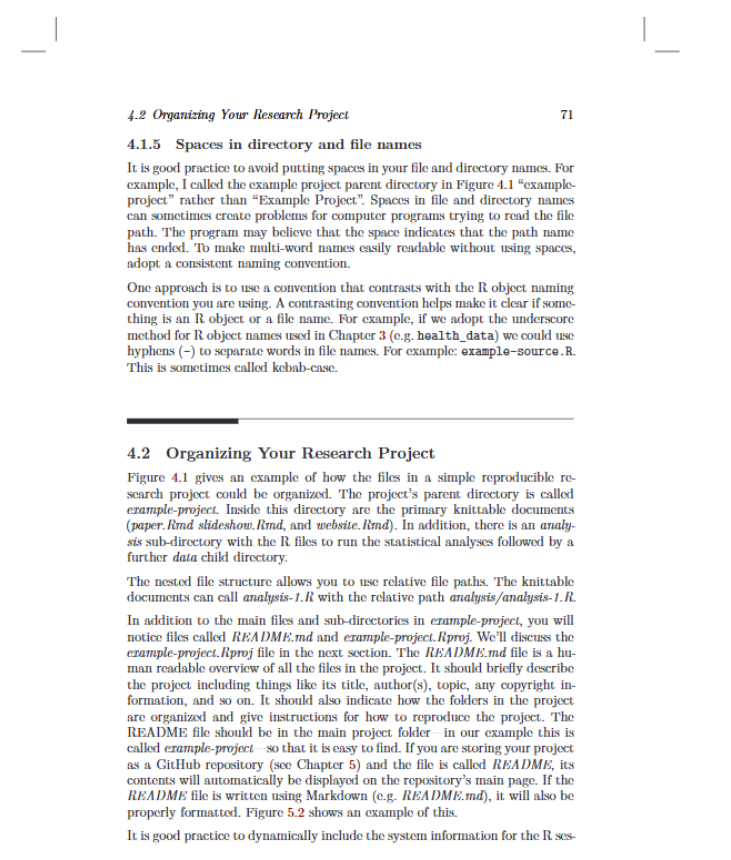
\includegraphics{images/clipboard-3489899846.png}



\end{document}
